% "Станет проще"

\documentclass[a4paper,12pt]{article} % тип документа

% report, book

% Рисунки
\usepackage{graphicx}
\usepackage{wrapfig}
\usepackage{hyperref}
\usepackage[rgb]{xcolor}
\pagestyle{plain}
\usepackage{floatflt}
\usepackage{multirow}
\usepackage{lipsum}
\usepackage{amsmath, amstext}
\usepackage{siunitx}
%\usepackage{subcaption}
\usepackage{wrapfig}
\usepackage{mathrsfs}
\usepackage{adjustbox}
\usepackage{enumerate, indentfirst, float}
\usepackage{pgffor}
\usepackage{capt-of, svg}
\usepackage{array}
\usepackage{longtable}
\usepackage{csvsimple}
\usepackage{pdfpages}
\usepackage{subfigure}
\usepackage{sectsty}



%  Русский язык

\usepackage[T2A]{fontenc}			% кодировка
\usepackage[utf8]{inputenc}			% кодировка исходного текста
\usepackage[english,russian]{babel}	% локализация и переносы



% Математика
\usepackage{amsmath,amsfonts,amssymb,amsthm,mathtools} 

\usepackage{wasysym}

%Заговолок
\author{Сафиуллин Роберт	}
\title{Лабораторная работа  4.3.2\\ Дифракция света на ультразвуковой волне в жидкости}





\begin{document} % начало документа

\maketitle


\newpage

\section{Цель работы:}
изучение дифракции света на синусоидальной акустической решетки и наблюдение фазовой решетки методом темного поля
\\
\section{В работе используются:}
оптическая скамья, осветитель, два длиннофокусных объектива, кювета с жидкостью,
кварцевый излучатель с микрометрическим винтом, генератор УЗ-частоты, линза, микроскоп.
 
        \section{Установка}
        \begin{center}
        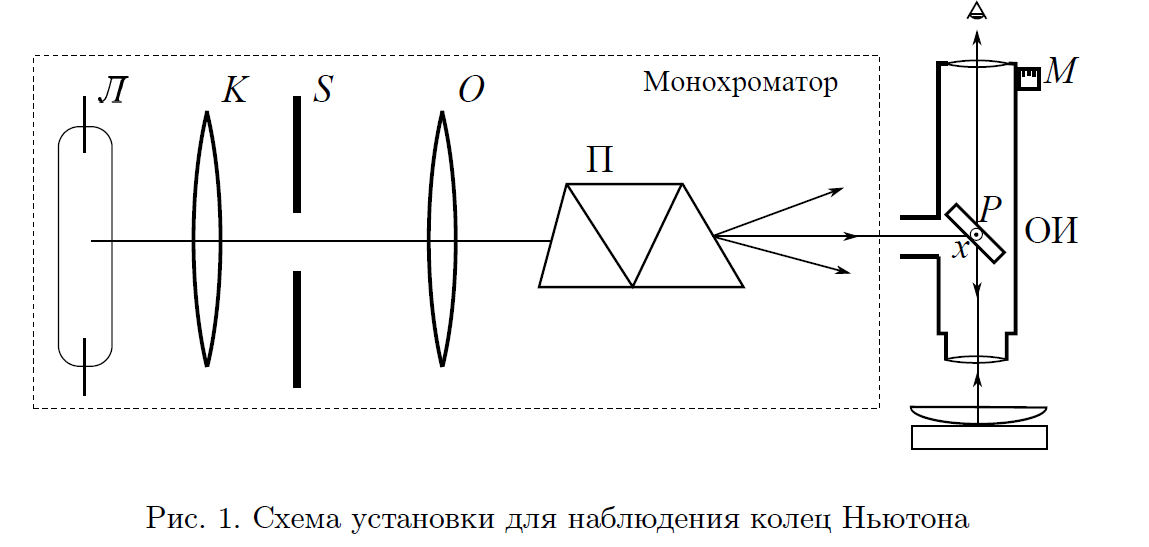
\includegraphics[scale=0.7]{ust}
        \end{center}


\section{Ход работы}
\textbf{Определение скорости ультразвука по дифракционной картине} \\
 1) Пoгрузили в жидкость излучатель Q на нужную глубину, такую, что на расстоянии от излучателя до противоположной стенки кюветы укладывалось целое число длин полуволн.\\
 2) Оценили таким способом длину волны $\Lambda$ как удвоенное расстояние между двумя наиболее интенсивными дифракционными картинами. \\
 Для УЗ-волны частоты $\nu = 1.076$ МГц длину волны $\Lambda$ = 2*65*10 = 1300 мкм.\\
 3) Используя формулу $v=\Lambda * \nu$ найдем скорость УЗ-волны в жидкости v = 1400 м/с ($v_{tabl}=1480$ м/с) \\
 4) Для разных частот определим координаты дифракционных полос. Результаты занесем в таблицу: \\
  \begin{center}

 \begin{tabular}{|c|c|c|c|}
 \hline 
 $\nu$, МГц & $y_{-1}$, мкм & $y_{0}$, мкм  & $y_{1}$, мкм  \\ 
 \hline 
 1.077 & -126 & 0 & 126 \\ 
 \hline 
 1.2 & -130 & 0 & 130 \\ 
 \hline 
 1.36 & -164 & 0 & 164 \\ 
 \hline 
 1.423 & -172 & 0 & 172 \\ 
 \hline 
 \end{tabular} 
 \end{center}
 
 5) Используя формулу $\Lambda=m*f*\frac{\lambda}{l_m}$, найдем $\Lambda$ ($\lambda = 640\pm20$ нм, f = 28 cm), а также $v$. Результаты занесем в таблицу:\\
 \begin{center}
 
 \begin{tabular}{|c|c|c|c|}
 \hline 
 $\nu$, МГц & $l_1$, мкм & $\Lambda$, мкм & v, м/c \\ 
 \hline 
 1.077  & 126 & $1422\pm44$ & $1531\pm47$ \\ 
 \hline 
 1.2  &130 & $1378\pm43$ & $1654\pm52$ \\ 
 \hline 
 1.36  &164 & $1093\pm34$ & $1487\pm46$ \\ 
 \hline 
 1.423  &172 & $1042\pm33$ & $1483\pm47$ \\ 
 \hline 
 \end{tabular} 
  \end{center}
\textbf{Определение скорости ультразвука методом темного поля}\\

 6) Разместим линзу между микроскопом и щелью, чтобы снова сделать пучок лучей параллельными.\\
 7) Откалибруем шкалу микроскопа с помощью квадратной сетки.(1мм = 23 деления шкалы) \\
 8) Установили ширину щели 30 мкм. \\
 9) Закрыли центральную гармонику проволокой, находящейся на расстоянии f от кюветы.\\
 10) Зафиксируем с помощью откалиброванной окулярной шкалы координаты первой и последней из хорошо видимых темных полос, а также их количество.(для разных частот )\\
 11) Результаты запишем в таблицy: \\
 \begin{center}
 
 \begin{tabular}{|c|c|c|c|c|}
 \hline 
 $\nu$ МГц & $\frac{1}{\nu}$ & r, mm & N, ед & $\Lambda$, мкм \\ 
 \hline 
 1.044 &0.96 &5.074 & 7 & 1450 \\ 
 \hline 
 1.058 & 0.95&4.191 & 6 & 1397 \\ 
 \hline 
 1.5 &0.67 &3.435 & 8 & 859 \\ 
 \hline 
 1.59 & 0.63&3.913 & 9 & 870 \\ 
 \hline 
 1.899 & 0.53&3.913 & 11 & 712 \\ 
 \hline 
 2.07 &0.48 &3.261 & 9 & 725 \\ 
 \hline 
 \end{tabular} 
 \end{center}

12) Построим график $\Lambda(\frac{1}{\nu})$\\
\begin{center}
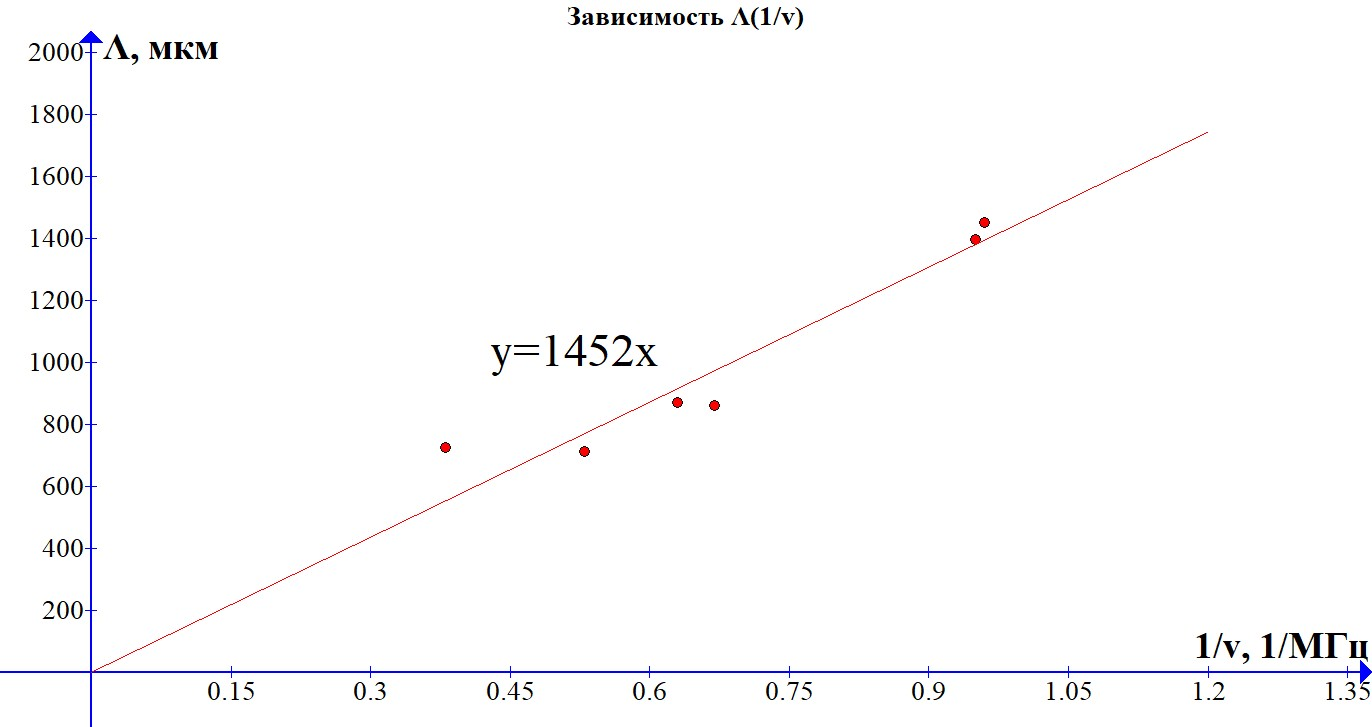
\includegraphics[scale=0.34]{25}
\end{center}
Отсюда скорость ультразвука в воде 1452 м/c($v_{tabl}=1480$ м/с)




















\end{document} % конец документа
